\documentclass[conference,a4paper,twoside]{IEEEtran}
\RequirePackage[T1]{fontenc}
\usepackage[utf8x]{inputenc}
\usepackage{lmodern}
\usepackage{cite}
\usepackage[ngerman]{babel}
\usepackage{amsmath,amssymb,amsfonts}
\usepackage{graphicx}
\usepackage{textcomp}
\usepackage{xcolor}
\usepackage{url}
\usepackage{float}
\usepackage{svg}
\def\BibTeX{{\rm B\kern-.05em{\sc i\kern-.025em b}\kern-.08em
    T\kern-.1667em\lower.7ex\hbox{E}\kern-.125emX}}
\begin{document}

\title{FEM-Hausarbeit: Automatisierung der Berechnung}

\author{
  \IEEEauthorblockN{Johannes Frielingsdorf}
  \IEEEauthorblockA{\textit{Fakultät für Informations-, Medien- und Elektrotechnik} \\
  \textit{Technische Hochschule Köln}\\
  Köln, Deutschland \\
  johannes.frielingsdorf@th-koeln.de}
}

\maketitle

%Polygone Afg. 1: 19642 nodes 32928 elements
%Polygone Afg. 2: 22162 nodes 37168 elements
%Polygone Afg. 3:

\section{Einführung}
In diesem Projekt wurde die Python Scripting-Schnittstelle von Agros2D verwendet, um systematisch Änderungen in der Simulationsgeometrie aus dem vorherigen Projekt des "Magnetischen Kreises" zu untersuchen.

Alle Simulationsdateien werden aufgabenweise als .zip-Archiv abgegeben, da im Rahmen der Projektbearbeitung mehrere Dateien pro Aufgabenstellung erstellt wurden. Dies umfasst sowohl mehrere Python-Skriptdateien, da in der Regel die Erstellung der Simulationsumgebung in eine eigene Datei ausgelagert wurde.

Da unter Ubuntu 20.04 offenbar matplotlib in Agros2D nicht verfügbar ist und auch eine Nachinstallation nicht gelang, wurde abweichend von der Aufgabenstellung jeweils eine .csv-Datei mit den Simulationsergebnissen durch Agros2D angelegt, die anschließend mit Gnuplot visualisiert wurde. Daher befindet sich in den jeweiligen Projektordnern eine .gnuplot-Datei zur Konfiguration des Plots, sowie Shellskripte zum Aufruf von Agros2D mit dem Python-Skript sowie Gnuplot.

Weiterhin steht das das Git-Repository des Projektes unter \url{https://github.com/bazjo/Agros2D-Automation} zur Verfügung.

\section{Aufgabenstellung 1}
In der ersten Aufgabenstellung wird der Elektromagnet aus Projekt 2 ohne Permanentmagnet erneut betrachtet. Es wird die magnetische Flussdichte im Luftspalt sowie die Anziehungskraft auf das I-Joch für verschiedene Stromstärken untersucht. Dazu wird eine Funktion zur Generierung einer halbseitigen Simulationsgeometrie unter Ausnutzung der Spiegelsymmetrie erstellt. Eine Simulation wird jeweils für Ströme von $1\ A$ bis $64\ A$ in $1\ A$-Schritten durchgeführt.

Dargestellt ist beispeilhaft eine Stromstärke von $64\ A$. Abb.~\ref{assignment_1_geometry} zeigt die Simulationsgeometrie, Abb.~\ref{assignment_1_mesh} das generierte Netz und Abb.~\ref{assignment_1_simulation} die resultierende Flussdichteverteilung. Die Netzknotenanzahl betrug in diesem Fall 19642; die Anzahl der Polygone 32928.

In dieser und in allen folgenden Aufgaben wurde stets, wo nicht anders angegeben, ein Verfeinerungsniveau und die Polynomordnung 2 verwendet.

\begin{figure}
\centerline{\includegraphics[width=0.7\columnwidth]{../assets/assignment_1_geometry.png}}
\caption{Simulationsgeometrie in der ersten Aufgabenstellung; $I = 64\ A$.}
\label{assignment_1_geometry}
\end{figure}

\begin{figure}
\centerline{\includegraphics[width=0.7\columnwidth]{../assets/assignment_1_mesh.png}}
\caption{Simulationsvermaschung in der ersten Aufgabenstellung; $I = 64\ A$.}
\label{assignment_1_mesh}
\end{figure}

\begin{figure}
\centerline{\includegraphics[width=0.7\columnwidth]{../assets/assignment_1_simulation.png}}
\caption{Flussdichteverteilung in der ersten Aufgabenstellung; $I = 64\ A$.}
\label{assignment_1_simulation}
\end{figure}

\begin{figure}
\centerline{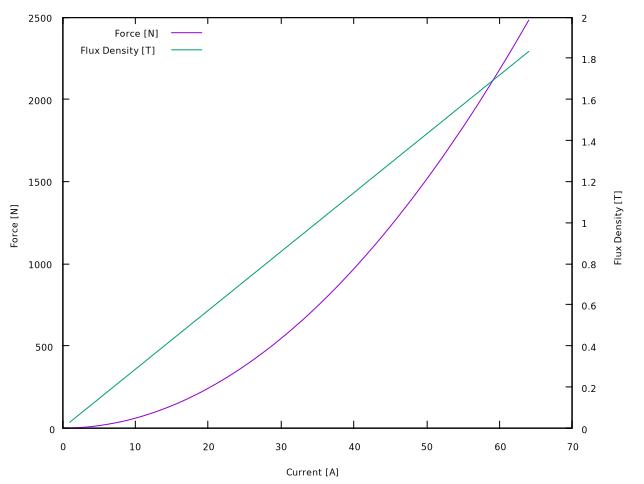
\includegraphics[width=\columnwidth]{../assets/assignment_1_plot.pdf}}
\caption{Kraft auf das I-Joch und Flussdichte im Luftspalt gegenüber Stromstärke.}
\label{assignment_1_plot}
\end{figure}

Für den in Projekt 2 zunächst simulierten Strom von $16\ A$ ergab sich dort eine Kraft auf das I-Joch von $162,96\ N$ (Aufgabe I.C.). Abweichend dazu ergab sich in dieser Simulation eine Kraft von $155,09\ N$, was einer Abweichung von etwa $4,8\ \%$ entspricht, der Wert liegt also in der erwarteten Größenordnung. Die beobachtete Abweichung kommt möglicherweise durch eine leicht andere Simulationgeometrie (runde vs. rechteckige Randbegrenzung, andere Dimensionen der Spule) zustande, außerdem konnte kein Weg gefunden werden, wie in Projekt 2 die Sollfläche der Polygone per Skript zu begrenzen.

Abb.~\ref{assignment_1_plot} zeigt einen Plot der Kraft auf das I-Joch und Flussdichte im Luftspalt für Ströme von $1\ A$ bis $64\ A$. Die bereits in Projekt 2, Aufgabe I.D. geäußerte Vermutung, dass $F \sim I²$ zeigt sich bestätigt. Für die Flussdichte im Lufspalt zeigt sich ein Zusammenhang $B \sim I$. Dies deckt sich mit dem aus der Physik bekannten Wissen, dass sich die mag. Flussdichte B einer Spule mit Länge l, Windungszahl N, Strom I und Kernmaterial mit $\mu_0$ durch

\begin{equation}
B = \mu_0 \cdot \mu_r \cdot {N \cdot I \over l}
\label{eq_magnetic_field_coil}
\end{equation}

beschreiben lässt.

Für die Kraft auf eine von der Flussdichte B durchflossene Grenzfläche A des magnetischen Kreises gilt dann

\begin{equation}
F = {1 \over 2} \cdot {B² \over \mu_0} \cdot A
\label{eq_electromagnetic_force}
\end{equation}

Die analytische Beschreibung des vorliegenden Problems entspricht also qualitativ dem beobachteten Simulationsergebnis.

\section{Aufgabenstellung 2}

Für die zweite Aufgabenstellung wird der Strom in der Spule zu Null gesetzt und der untere Teil des U-Joches durch ein permanentmagnetisches Material mit $\mu_r = 1,11$ und der Remanenzflussdichte $B = 1,28\ T$ ersetzt, welches im der parametrischen Modellgenerierung mit variabler Dicke erstellt werden kann. Zunächst wird eine Dicke von $3\ mm$ betrachtet, anschließend eine variable Dicke von $1 - 11\ mm$.

Dargestellt ist beispeilhaft eine Dicke d von $11\ mm$. Abb.~\ref{assignment_2_geometry} zeigt die Simulationsgeometrie, Abb.~\ref{assignment_2_mesh} das generierte Netz und Abb.~\ref{assignment_2_simulation} die resultierende Flussdichteverteilung. Die Netzknotenanzahl betrug in diesem Fall 22162; die Anzahl der Polygone 37168.

\begin{figure}[H]
\centerline{\includegraphics[width=0.7\columnwidth]{../assets/assignment_2_geometry.png}}
\caption{Simulationsgeometrie in der zweiten Aufgabenstellung; $d = 11\ mm$.}
\label{assignment_2_geometry}
\end{figure}

\begin{figure}[H]
\centerline{\includegraphics[width=0.7\columnwidth]{../assets/assignment_2_mesh.png}}
\caption{Simulationsvermaschung in der zweiten Aufgabenstellung; $d = 11\ mm$.}
\label{assignment_2_mesh}
\end{figure}

\begin{figure}[H]
\centerline{\includegraphics[width=0.7\columnwidth]{../assets/assignment_2_simulation.png}}
\caption{Flussdichteverteilung in der zweiten Aufgabenstellung; $d = 11\ mm$.}
\label{assignment_2_simulation}
\end{figure}

\begin{figure}[H]
\centerline{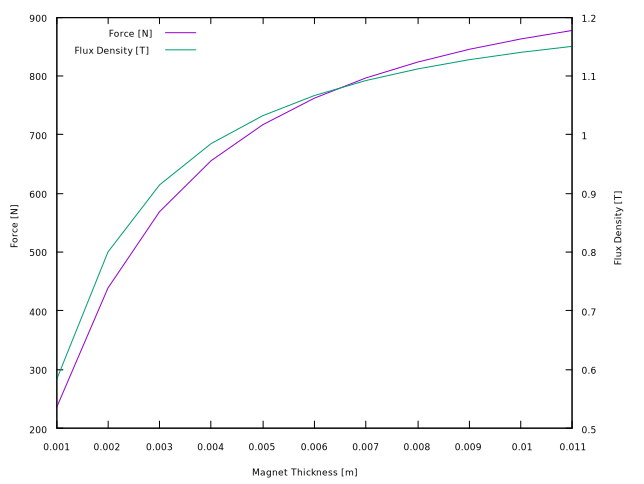
\includegraphics[width=\columnwidth]{../assets/assignment_2_plot.pdf}}
\caption{Kraft auf das I-Joch und Flussdichte im Luftspalt gegenüber Dicke des Permanentmagneten.}
\label{assignment_2_plot}
\end{figure}

Für eine Dicke $d = 3\ mm$ des permanentmagnetischen Material ergibt sich eine Anziehungskraft $F = 568,69\ N$ sowie eine Flussdichte im Spalt $B = 0,914\ T$.

Da in diesem Projekt nicht mit Magnetisierungskurven und auch sonst mit leicht anderen Werten gearbeitet wurde, ist kein direkter Vergleich der Werte mit den ensprechenden aus Projekt 2, Aufgabe II.B. möglich.

Bei Betrachtung des Verlaufs der Kraft auf das I-Joch und Flussdichte im Luftspalt für Dicken von $1\ mm$ bis $11\ mm$ in Abb.~\ref{assignment_2_plot} zeigt sich jedoch qualitativ das gleiche Verhalten wie in Projekt 2; auch hier strebt die Flussdichte und nach Gl.~(\ref{eq_electromagnetic_force}) die Kraft asymptotisch gegen ein Maximum.

Dieses Verhalten ergibt sich aus der Hysterese des ferromagnetischen Material des Permanentmagneten, dass durch die Angabe der Remanenzflussdichte in der Simulation angegeben wurde. Hierdurch bedingt gerät das Material in eine magnetische Sättigung, in der eine Erhöhung der magnetischen Feldstärke H nicht mehr linear eine Erhöhung der magnetischen Flussdichte bewirkt.

\end{document}
